\documentclass[11pt,letterpaper]{article}
\usepackage[utf8]{inputenc}
\usepackage[spanish]{babel}

\selectlanguage{spanish}
\usepackage{amsmath}
\usepackage{amsfonts}
\usepackage{amssymb}
\usepackage{fancyhdr, graphicx}
\pagenumbering{gobble}
\usepackage{subcaption}
\usepackage{float}

\usepackage{wrapfig}
\usepackage[T1]{fontenc}
\renewcommand{\headrulewidth}{0pt}
\usepackage{multicol}

\pagestyle{plain}
\usepackage[left=2cm,right=2cm,top=2cm,bottom=2cm]{geometry}
\author{}
\date{}
\title{Plan de trabajo}

\begin{document}
\begin{wrapfigure}{l}{4cm}
    \centering
    \vspace{-2cm}
   \hspace{-2cm} 
\includegraphics[width=4cm]{logo.png}
\end{wrapfigure}

\hspace{2cm} \textbf{Reporte de trabajo} \hfill \\
\flushright{Ciudad universitaria a 21 de septiembre del 2022.}\\
\flushleft{\textbf{A la Comisión de Servicio Social de la Licenciatura en Física Biomédica.} }\\
\vspace{-0.5cm}
\flushleft{\textbf{Facultad de Ciencias}}\\
\vspace{-0.5cm}
\flushleft{\textbf{Universidad Nacional Autónoma de México}}\\
\hfill \\
\begin{flushleft}
\hspace{2cm} Por este medio comunico un reporte de las actividades que realicé para validar mi Servicio Social en la \textbf{Facultad de Ciencias} en el programa Apoyo a la docencia y asesoría académica (Prácticas computacionales y manuales experimentales para la enseñanza de  Electrofisiología), con clave 2022-12-12-1269, registrado ante DGOAE, cubriendo un total de 480 horas, del 14 de febrero al 20 de septiembre del 2022.\\
\hfill \\
\textbf{Febrero-marzo:} En estos meses leí el material didáctico que ya estaba disponible en el repositorio de GitHub previo (\href{https://github.com/emckiernan/electrophys}{https://github.com/emckiernan/electrophys}). Había datos que ya estaban analizados, pero la mayor parte del repositorio contenía datos sin procesar o datos a los cuales se les podía extraer mucha más información. A la par del análisis del material de GitHub, busqué en publicaciones nuevos algoritmos computacionales para la extracción de datos electrofisiológicos. Con toda esta información generé 4 propuestas de notebooks.  \\
\hfill \\
\textbf{Abril-junio:} En este periodo escribí un código de análisis de ECG que filtraba datos y extraía las ondas PQRST. Primero se hizo un filtrado de las señales y se estandarizaron criterios de exclusión de mediciones. Luego se hizo un análisis de frecuencias para encontrar los picos R. A partir de esta onda, se obtuvieron los marcadores de las ondas P, Q, S y T. Después se obtuvieron distancias y segmentos importantes para el diagnóstico de patologías cardíacas, y se evaluó la variación de estos parámetros durante toda la medición. Con todo esto desarrollé un algoritmo que automáticamente hacía la extracción de parámetros de una grabación de ECG.  Este algoritmo se aplicó una base de datos de pacientes con arritmias y los datos extraídos fueron alimentados a una red neuronal convolucional de tres capas. Se hicieron varias pruebas con los hiperprarámetros de las pruebas y se mostró cómo evaluar una estructura.  \\
\begin{figure}[H]
\centering
\begin{minipage}{.48\linewidth}
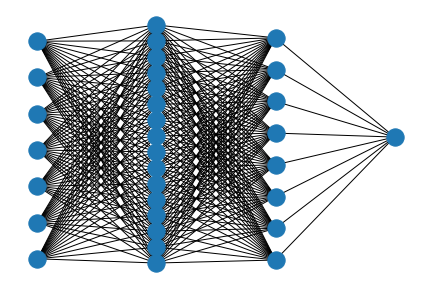
\includegraphics[width=\linewidth]{../../../GitHub/Servicio_social/ECG/Images/Arq.png} 
\caption{\footnotesize{Estructura de la red neuronal convolucional usada para detectar arritmias en mediciones de ECG.}}
\label{arq}
\end{minipage}
\hfill
\begin{minipage}{.48\linewidth}
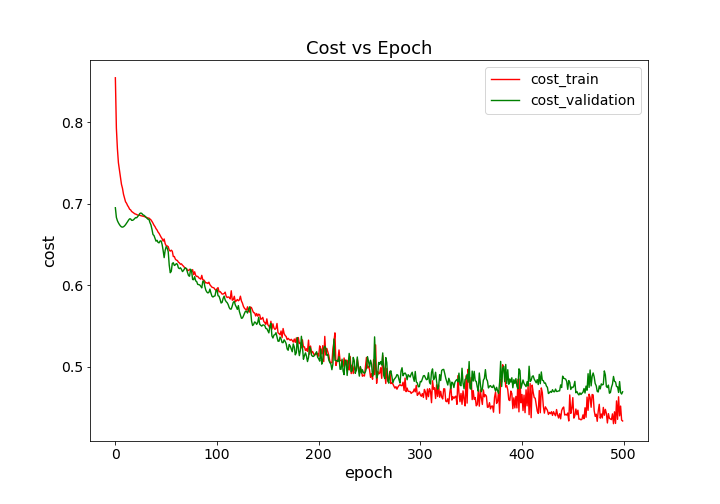
\includegraphics[width=\linewidth]{Build.png} 
\vspace{-0,8cm}
\caption{\footnotesize{Evolución de la función de costo(entropía cruzada binaria) con cada época de entrenamiento.}}
\label{build}
\end{minipage}
\end{figure}
\hfill 
\\Exploré diferentes estructuras y evalué cada arquitectura de red hasta encontrar la óptima para identificar arritmias. El algoritmo final obtuvo una precisión de 75\% (en el conjunto de validación). De los resultados también cabe recalcar que se logró una sensibilidad de 87.5\%. La forma en la que se desarrolló y evaluó tanto la arquitectura como el algoritmo en general, el lector será capaz de usar y ajustar redes neuronales convolucionales para resolver otros problemas usando este repositorio como guía. Estos notebooks se pueden ver en la carpeta de ECG: \href{https://github.com/Javi-ciencias/Servicio_social/tree/main/ECG/Code}\\
\hfill \\

\textbf{Julio:}  Utilicé los datos de espirometría con EMG de la base de datos y escribí un código de visualización de los datos, así como un pequeño análisis en el que se compara la amplitud de la señal muscular con el flujo de aire durante una expiración forzada. Dado que se contaban con pocos datos, no se pudo hacer un análisis más profundo. Adicionalmente, se trabajó con datos de EMG de antebrazo durante actividad intermitente. A estos datos se les hizo un análisis de EMG estandar, explicado y desarrollado por pasos. Finalmente, se realizó un análisis de PSD para observar el reclutamiento de fibras con pulsos de diferentes intensidades. \\
\hfill \\
\textbf{Agosto-septiembre:} Encontré unos datos de libre acceso en la base de \textbf{openneuro.org}. Los datos corresponden a un estudio de pacientes pediátricos con epilepsia en el que se realizaron registros de EEG durante el sueño. Estos datos son visualizados y explorados, paso a paso. Posteriormente, se explican las bases fisiológicas de la práctica para proponer conjuntos de parámetros que pueden servir para caracterizar adecuadamente un segmento de 10 segundos. Luego escribí un algoritmo de clústers por optimización de desviaciones estándar con estos conjuntos de parámetros. Usé varias técnicas de aprendizaje supervisado y expliqué paso a paso cada una. \\
\hfill \\
\begin{figure}[H]
\centering
\begin{minipage}{.48\linewidth}
\vspace{2cm}
	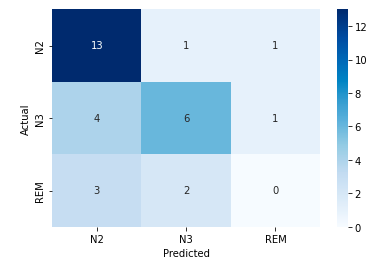
\includegraphics[width=0.9\linewidth]{confusion.png}
	\vspace{1.2cm}
	\caption{\footnotesize{ Matriz de confusión del algoritmo final usando un método de agrupación por vecinos (\textit{k-neighbor}). Estos resultados corresponden al conjunto de validación.}}
	\label{confusion}
\end{minipage}
\hfill
\begin{minipage}{.48\linewidth}
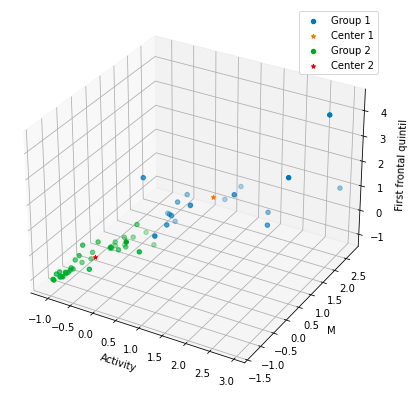
\includegraphics[width=\linewidth]{Disp.png} 
\caption{\footnotesize{Dispersión en 3D de los datos clasificados en dos clusters con sus respectivos centroides.}}
\label{disp}
\end{minipage}
\end{figure}
Utilicé y expliqué algoritmos de K-means que funciona con centroides de clústers y optimización de desviaciones estándar, así como con algoritmos de clasificación por vecinos y algoritmos de \textit{Support vector machine} que funcionan con hiperplanos de división entre conjuntos. Se logró obtener un algoritmo de clasificación de etapas de sueño con una precisión del 61.2\% que, por problemas de sesgo en los datos, no se pudo mejorar. En la figura \ref{confusion} se puede observar que la proporción de segmentos en cada etapa tiene una clara carga hacia la primeras etapas de sueño. Esto hace que el algoritmo tienda a clasificar los segmentos como NREM, por lo tanto tiene dificultades para identificar los segmentos REM. \\
\hfill \\
Finalmente, se identificaron dos grupos de datos para las etapas de sueño N2 y N3 alrededor de dos centroides. En la figura \ref{disp} se puede observar unsa dispersión en 3D de los centroides con sus respectivos conjuntos de datos. También se puede observar cómo los elementos del grupo 2 se agrupan de forma compacta, mientras que los elementos del grupo 1 parecen tener aberraciones o anormalidades que se separa mucho de la media. Se deja como trabajo futuro un estudio que valide si uno de los dos grupos coincide con mediciones durante un ataque epiléptico.\\
 \hfill \\
Todo el material es de libre acceso y se puede consultar en un repositorio de GitHub en la siguiente liga: \href{https://github.com/Javi-ciencias/Servicio\_social}. \\
\hfill \\
\end{flushleft}
\begin{multicols}{2}
 \begin{center}
\textbf{Atentamente} \\
\hfill \\
\hfill \\
\hfill \\
\hfill \\
\hfill \\
\rule{7cm}{0.4pt}\\
\textbf{Javier Serrano Molina}\\
\end{center}
 \columnbreak
 \begin{center}
\textbf{Visto bueno} \\
\hfill \\
\hfill \\
\hfill \\
\hfill \\
\hfill \\
\rule{7cm}{0.4pt}\\
\textbf{Dra. Erin Christy McKiernan}\\
\textbf{Profesora de Carrera Asociado C.}\\
\textbf{Departamento de física, Facultad de Ciencias, UNAM}
\end{center}
\end{multicols}

\end{document}